\documentclass[11pt]{article}
\usepackage{amsmath, amssymb, amscd, amsthm, amsfonts}
\usepackage{graphicx}
\usepackage{hyperref}
\usepackage{commath}
\usepackage{subfig}
\usepackage{float}
\oddsidemargin 0pt
\evensidemargin 0pt
\marginparwidth 40pt
\marginparsep 10pt
\topmargin -20pt
\headsep 10pt
\textheight 8.7in
\textwidth 6.65in
\linespread{1.5}

\title{Comparison on Algorithms for Vertex Cover Problem}
\author{Tiankai Jiang \and Chuxi Zhang}
\date{\today}

\newtheorem{theorem}{Theorem}
\newtheorem{lemma}[theorem]{Lemma}
\newtheorem{conjecture}[theorem]{Conjecture}

\newcommand{\rr}{\mathbb{R}}

\newcommand{\al}{\alpha}
\DeclareMathOperator{\conv}{conv}
\DeclareMathOperator{\aff}{aff}

\makeatletter
\setlength{\@fptop}{0pt}
\makeatother
\bibliographystyle{ieeetr}
\begin{document}

\maketitle

\begin{abstract}
This paper presents the reduction of Vertex Cover Problem to CNF Satisfiability Problem using a naive encoding method and sequential counter encoding, then it presents the comparison on time efficiency and approximate ratio between the exact solution of Vertex Cover using $miniSAT$ and two of the approximate solutions.
\end{abstract}
\section{Introduction}\label{section-introduction}
\textbf{The Vertex Cover Problem:} given a graph $G=(V,E)$, a positive integer $K\leq \abs{V}$, $\exists V'\subseteq V,$\linebreak$\abs{V'} \leq K, \forall \{u,v\}\in E: \{u,v\}\cap V' \neq \emptyset$?\\
\textbf{The CNF-SAT Problem:} given a boolean formula $f(x_1,\ldots ,x_n)$ in conjunctive normal form, is $f$ satisfiable? 

Cook–Levin theorem\cite{Cook:1971:CTP:800157.805047} states that Boolean Satisfiability Problem(\textbf{SAT}) is NP-complete. By reducing the SAT problem to CNF-SAT problem, we can prove the latter is also NP-complete. And by reducing CNF-SAT to Clique problem, which can be further reduced to Vertex Cover Problem, we know the Vertex Cover Problem is NP-complete as well. Hence, Vertex Cover Problem can be solved using a SAT solver by reducing it to CNF-SAT Problem.

\section{The Reduction}\label{section-reduction}
Given a graph $G=(V,E)$, let $n=\abs{V}$, let $x_i\{0, 1\}, i \in n$ denote if the $ith$ vertex is in the vertex cover, for a vertex cover of $k$ vertices, two conditions must be met\cite{Stamm-wilbrandt93programmingin} for a valid reduction:
\begin{itemize}
  \item For an arbitrary $e\langle u,v\rangle \in E$, at least one of $\{x_u,x_v\}$.
  \item $\sum\limits_{i=1}^{n}x_i\leq k$
\end{itemize}

The first condition ensures that at least one vertex of an edge is selected therefore that edge is covered. And the second condition, which is called boolean cardinality constraint, ensures that there are at most k vertices selected.

It is straightforward to express the first condition in conjunctive normal form:\[\bigwedge\limits_{\langle u,v\rangle \in E} x_u \lor x_v \]

But it is not that easy for the second one. In fact, the encoding of cardinality constraint has a great impact on the performance of the SAT solver, which we will discuss in the next section.

\section{Encoding of Boolean Cardinality Constraints}\label{section-encoding}
We will present the sequential counter encoding\cite{10.1007/978-3-030-30446-1_7,10.1007/11564751_73} and its advantage over the encoding given in ece650.a4.
\subsection{The Sequential Counter Encoding}
Given $x_1\ldots x_n$, the encoding introduces an extra of $(n-1)*k$ variables, denoted $s_{i,j}$, where $i \in [1,n-1], j\in [1,k]$. The $k$ variables in $s_{i,*}$ represent the number of variables in $x_1\ldots x_n$ that are true in base 1.
\begin{figure}[H]
\centerline{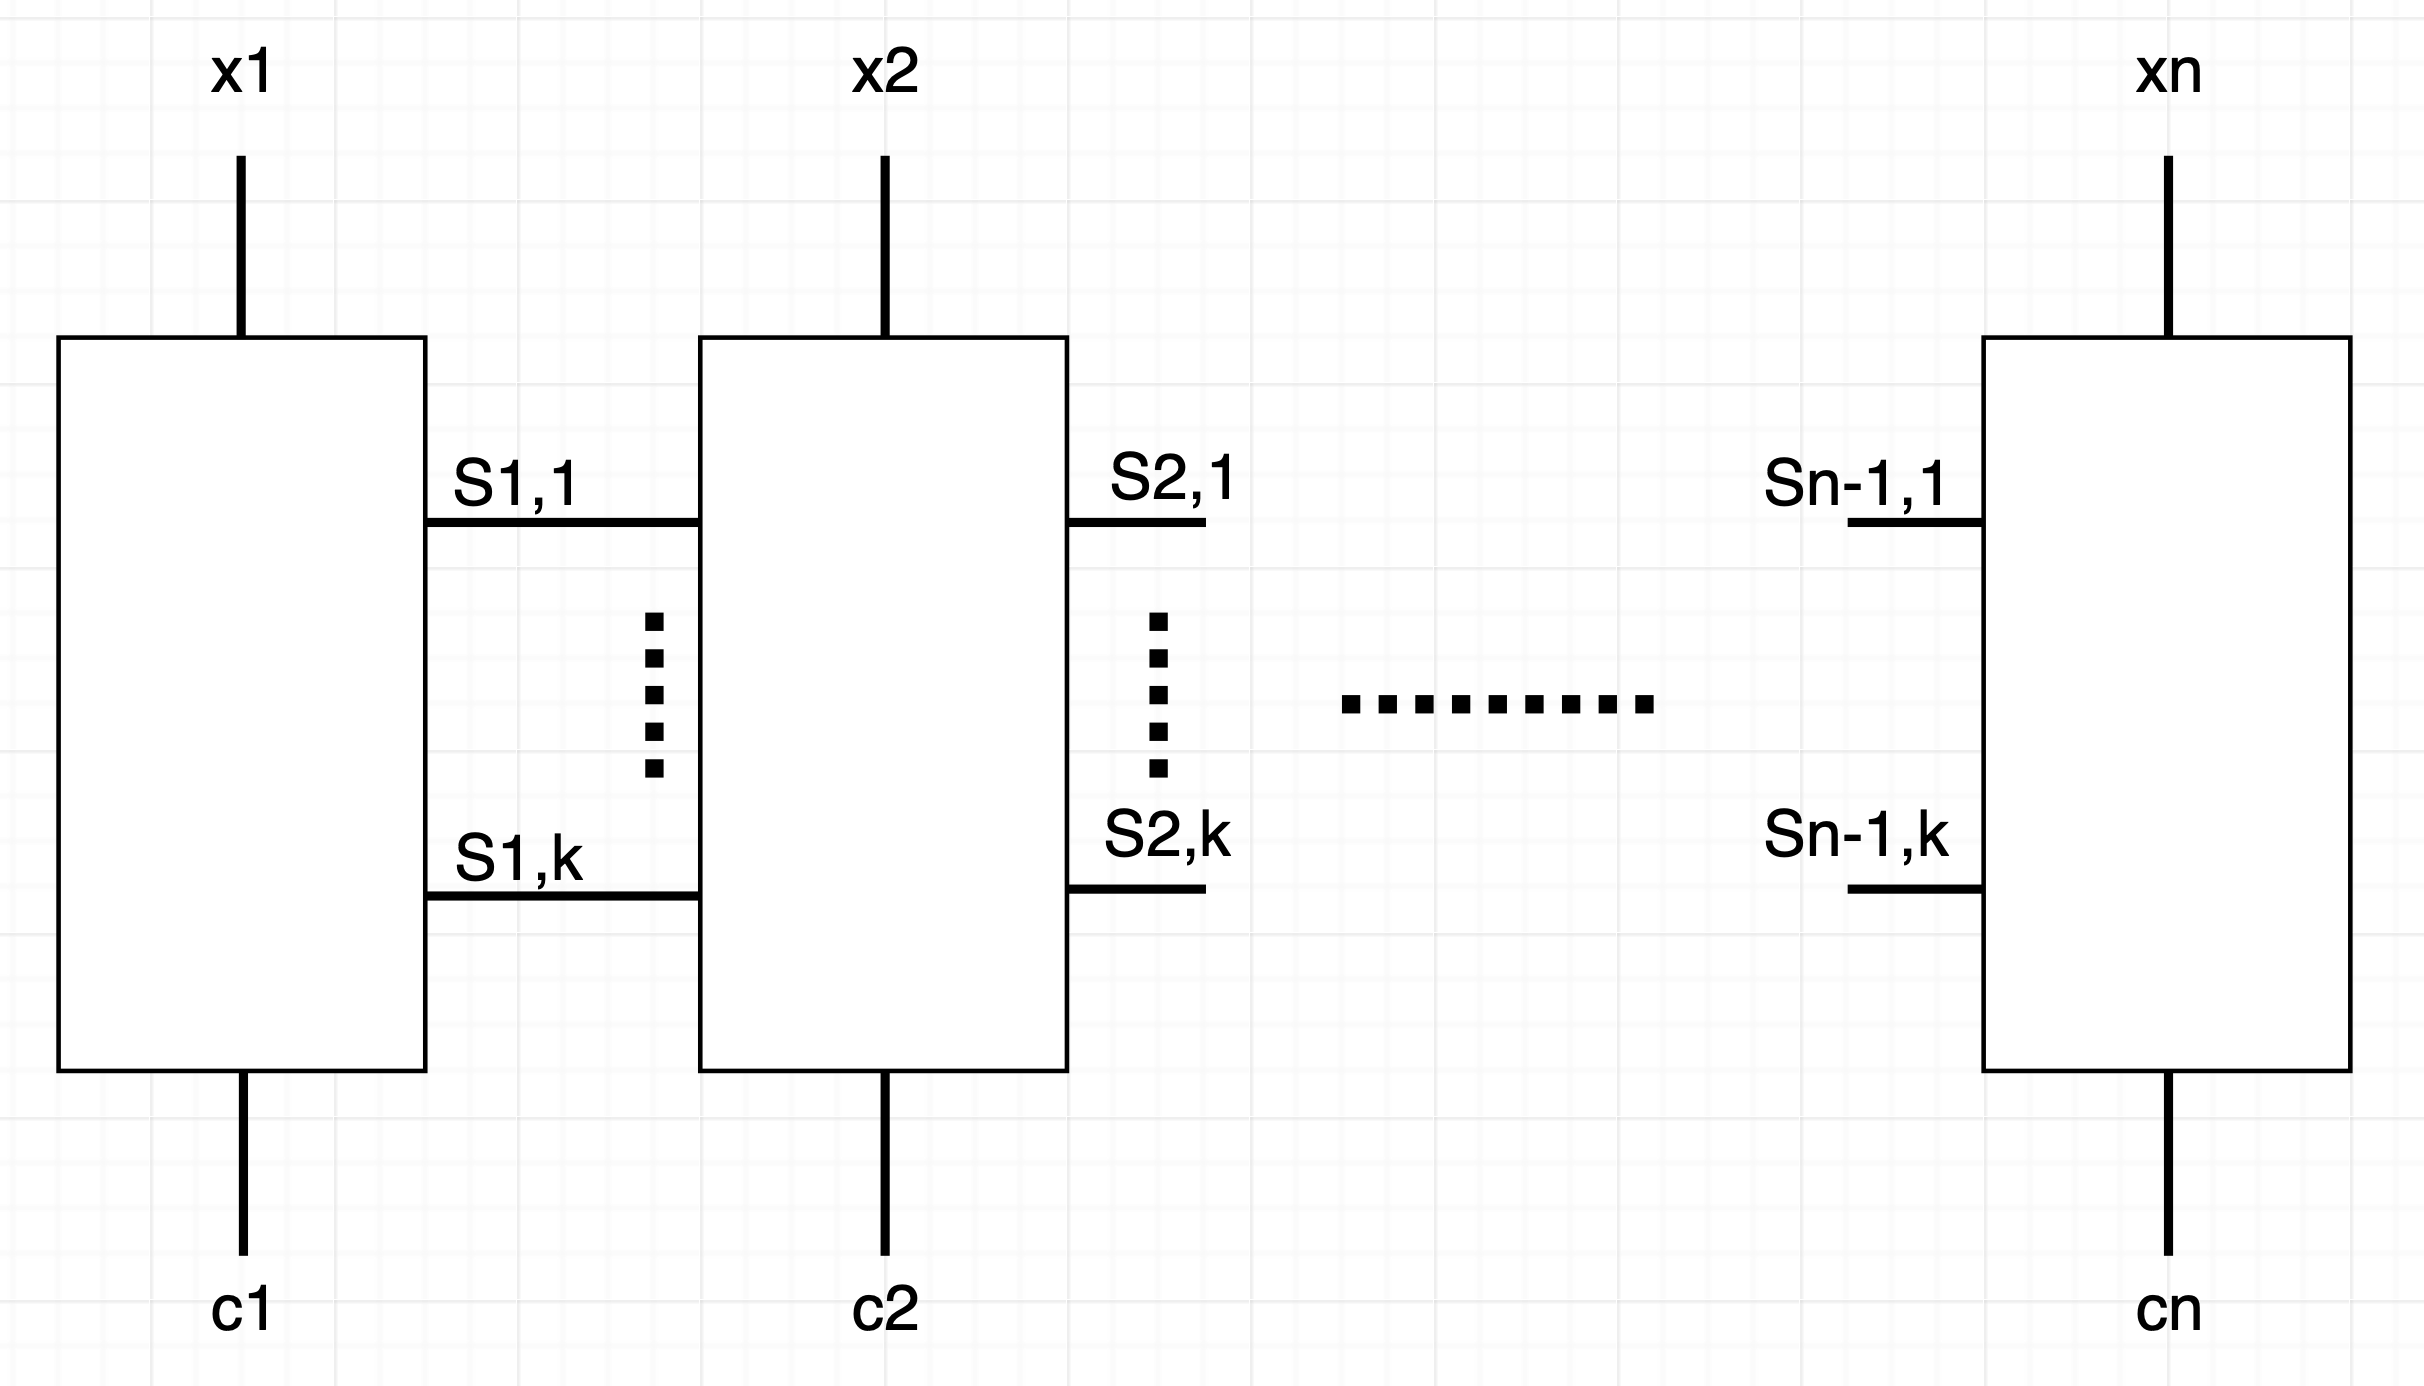
\includegraphics[width=11cm]{circuit.png}}
\caption{The Sequential Counter Circuit}
\end{figure}
\begin{figure}[H]
    \centering
    \subfloat[Sub-circuit of the sequential counter]{{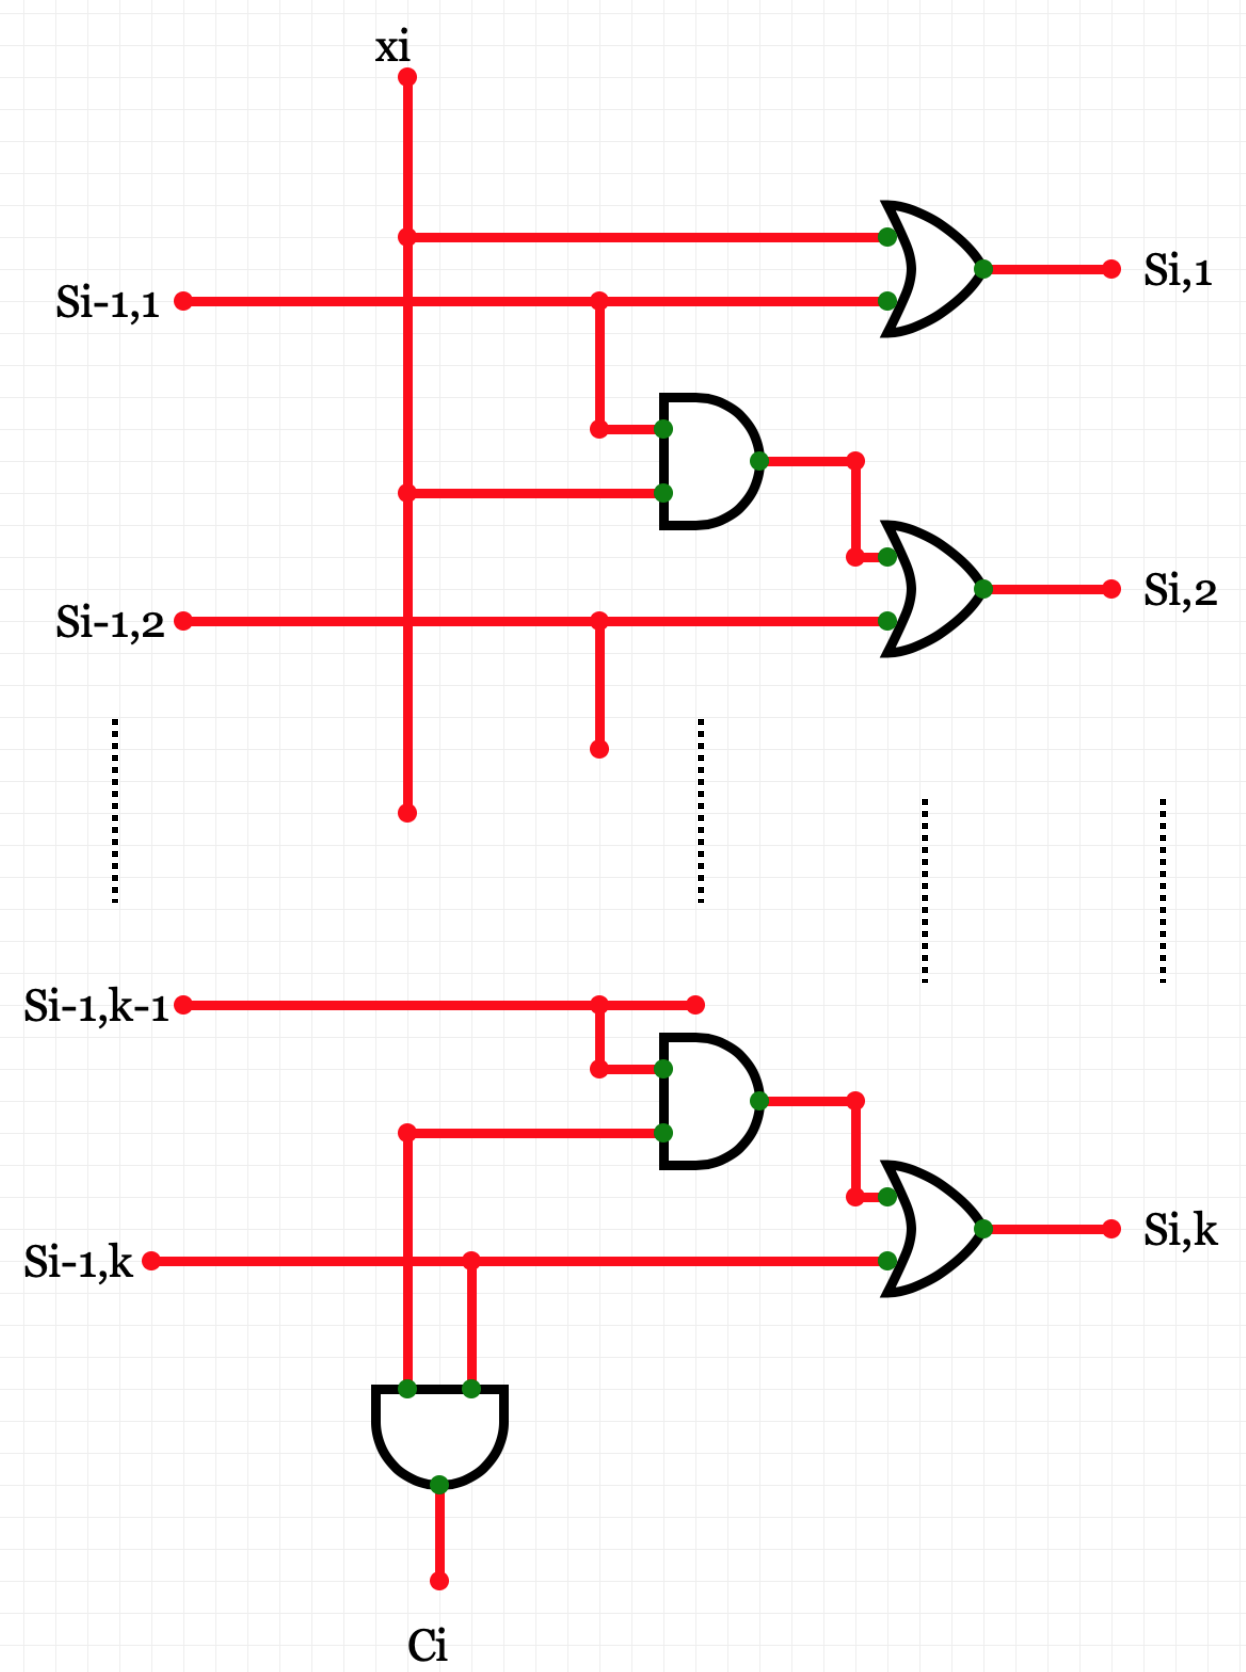
\includegraphics[width=7cm]{subcircuit.png} }}%
    \qquad
    \subfloat[Demo counting using a 4 bits input]{{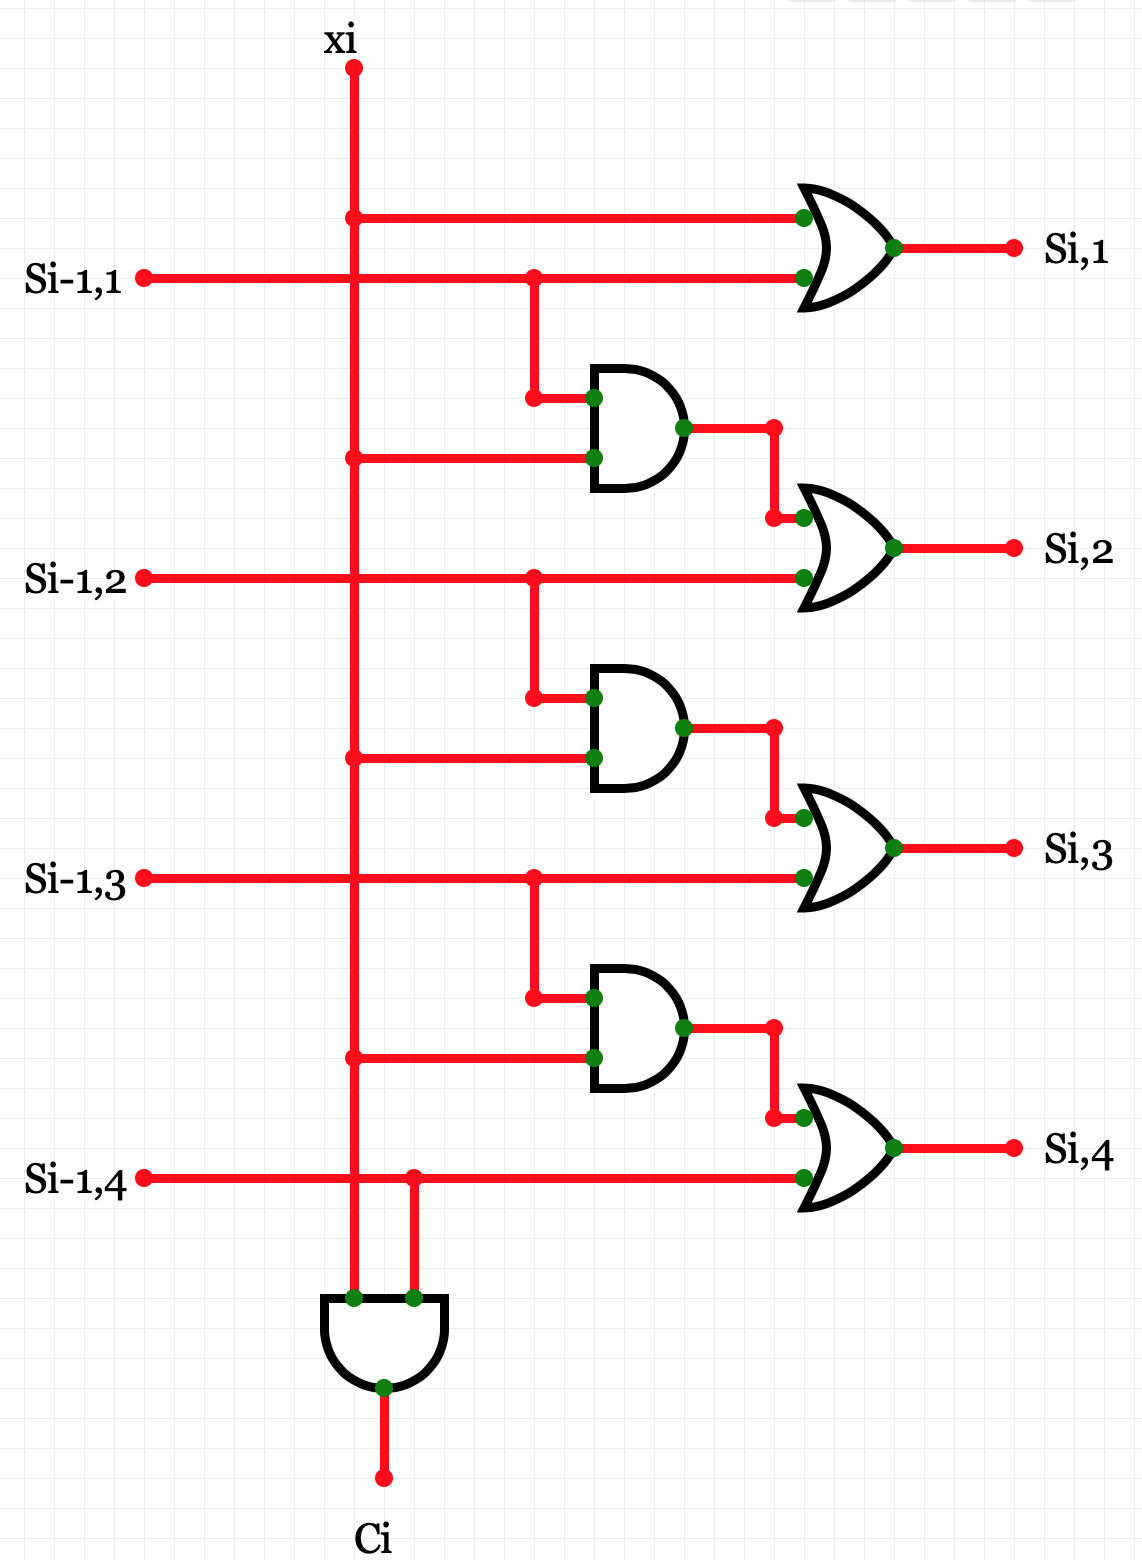
\includegraphics[width=7cm]{demoadd.png} }}%
    \caption{Sub-circuits}%
\end{figure}

Figure 1 shows the sequential counter circuit. Initially, the counter is set to 0. And the circuit will count the number of 1 in $x_1\ldots x_n$. As long as the overflow bit $c_i$ is not 1, $\sum\limits_{i=1}^{n}x_i\leq k$ holds.

Figure 2(a) shows the implementation of the sub-circuit in Figure 1. The sub-circuit takes a number in base 1 from [$s_{i-1,1}$, $s_{i-1,k}$], add $x_i(0\;or\;1)$ and output the results as a number in base 1 to [$s_{i,1}$, $s_{i,k}$]. Figure 2(b) shows a demo when $k=4$. Suppose the input is 2(1100 in unary), and $x_i$ is 1, after the addition, the output will be 3(1110 in unary). If the input is 4(1111) instead, after adding $x_i=1$, the overflow bit $c_i$ is 1 and we will know that the result exceeds 4.

The encoding are as follows:

Since $x_i$ connects directly to an $OR$ gate in each sub-circuit, $s_{i,1}$ must be 1 if $x_i$ is 1.\[\bigwedge\limits_{i=1}^{n-1} \neg x_i \lor s_{i,1}\]

Since there is no input in the first sub-circuit, the output of it is at most 1, which means $s_{1,2}$ to $s_{1,k}$ are guaranteed to be 0.\[\bigwedge\limits_{i=2}^{k} \neg s_{1,i}\]

Since $s_{i-1,j}$ connects directly to an $OR$ gate in each sub-circuit, $s_{i,j}$ must be 1 if $s_{i-1,j}$ is 1.\[\bigwedge\limits_{i=2}^{n-1}\bigwedge\limits_{j=1}^{k}\neg s_{i-1,j} \lor s_{i,j}\]

Since $x_i$ and $s_{i-1,j-1}$ are connected to a $AND$ gate and then the $AND$ gate connects to an $OR$ gate, $s_{i,j}$ must be 1 if $x_i$ and $s_{i-1,j-1}$ are both 1.\[\bigwedge\limits_{i=2}^{n-1}\bigwedge\limits_{j=2}^{k}\neg x_i\lor\neg s_{i-1,j-1} \lor s_{i,j}\]

There should not be any overflow in all n sub-circuits.($i$ starts from 2 because there is no input for the first sub-circuit).\[\bigwedge\limits_{i=2}^{n-1}\neg x_i\lor\neg s_{i-1,k}\]

\subsection{Encoding Efficiency}
The encoding method to represent cardinality constraint in ece650.a4 uses in total $n*k$ atomic propositions and $k+n{k\choose 2}+k{n\choose 2}$ clauses. The sequential counter encoding also uses $(n-1)*k+n$ atomic propositions, and in total $(n+1)+(k-1)+k(n-2)+(k-1)(n-2)+(n-2)=2nk+n-3k-2$ clauses. In the worst case, when $n=k$, the naive encoding uses $n^3-n^2+n$ clauses while the sequential counter uses only $2n^2-2n-2$ clauses, which is significantly better than the previous one. When $k=\frac{n}{2}$, the former uses $\frac{3n^3-4n^2+4n}{8}$ clauses while the latter uses $\frac{2n^2-n-4}{2}$ clauses. The sequential counter is still much better.
\section{Approximation Algorithms}\label{section-approx}
For a NP-complete problem, an exponential running time algorithm for an exact soluton is expected. To reduce the time complexity, approximate solutions are considered. We apply greedy algorithm and random algorithm on Vertex Cover Problem.
\subsection{The Greedy Algorithm}
Choose a vertex with highest degree each time and remove all its edges until no edge remains. The time complexity is $O(\abs{V}+\abs{E})$. Assume set $C$ contains the vertices the algorithm chooses, $m$ is the number of vertices in the optimal solution and $H_m$ the Harmonic series. \[\abs{C} = \sum_{i = 2}^{m}\abs{C_i}=\sum_{i = 2}^{m}\left \lfloor \frac{m}{i} \right \rfloor\geq\sum_{i = 2}^{m}(\frac{m}{i} - 1)\geq m\sum_{i = 1}^{m}\frac{1}{i} - 2m = m(H_m - 2)\]
$\frac{\abs{C}}{\abs{C^*}}=\frac{m(H_m - 2)}{m}=H_m - 2=\Omega(\log(n))$ And we get its upper bound by set cover problem.\cite{Cormen:2009:IAT:1614191}. Hence, this is a $\theta(\log(n))$-approximation algorithm.
\subsection{The Random Algorithm}
Randomly choose an edge each time and remove both of its vertices' edges until no edge remains. The time complexity is $O(\abs{V}+\abs{E})$(adjacency list representation). Assume that set $A$ includes all the edges chosen. Every time we can put two vertices into vertex cover set $C$. Hence, $\abs{C} = 2\abs{A}$. Assume $C^*$ is the optimal solution, which must cover A. For no edges in $A$ share a common vertex and $C^*$ includes at least one vertex of each edge in $A$, $\abs{A}\leq\abs{C^*},\abs{C}=2\abs{A}\leq2\abs{C^*}, \frac{\abs{C}}{\abs{C^*}}\leq 2$. Hence, this is a 2-approximation algorithm\cite{Cormen:2009:IAT:1614191}.
\section{Performance Evaluation}\label{section-experiment}
\subsection{Experiment Setup}
Randomly generate 10 graphs for each $\abs{V} \in [5,50]$ in increment of 5 and test the CNF-SAT(two encodings) and two approximate algorithms with each graph for 10 times. Calculate mean and standard deviation of running time for each $\abs{V}$ for all four algorithms(CNF-SAT with two encoding methods) and calculate approximate ratio for the two approximate algorithms. Randomly generate 10 graphs for each $\abs{V} \in [50,2000]$ in increment of 25 and test two approximate algorithms. Calculate the average run time and vertices selected.
\subsection{Experiment Result}
\begin{figure}[H]
\centerline{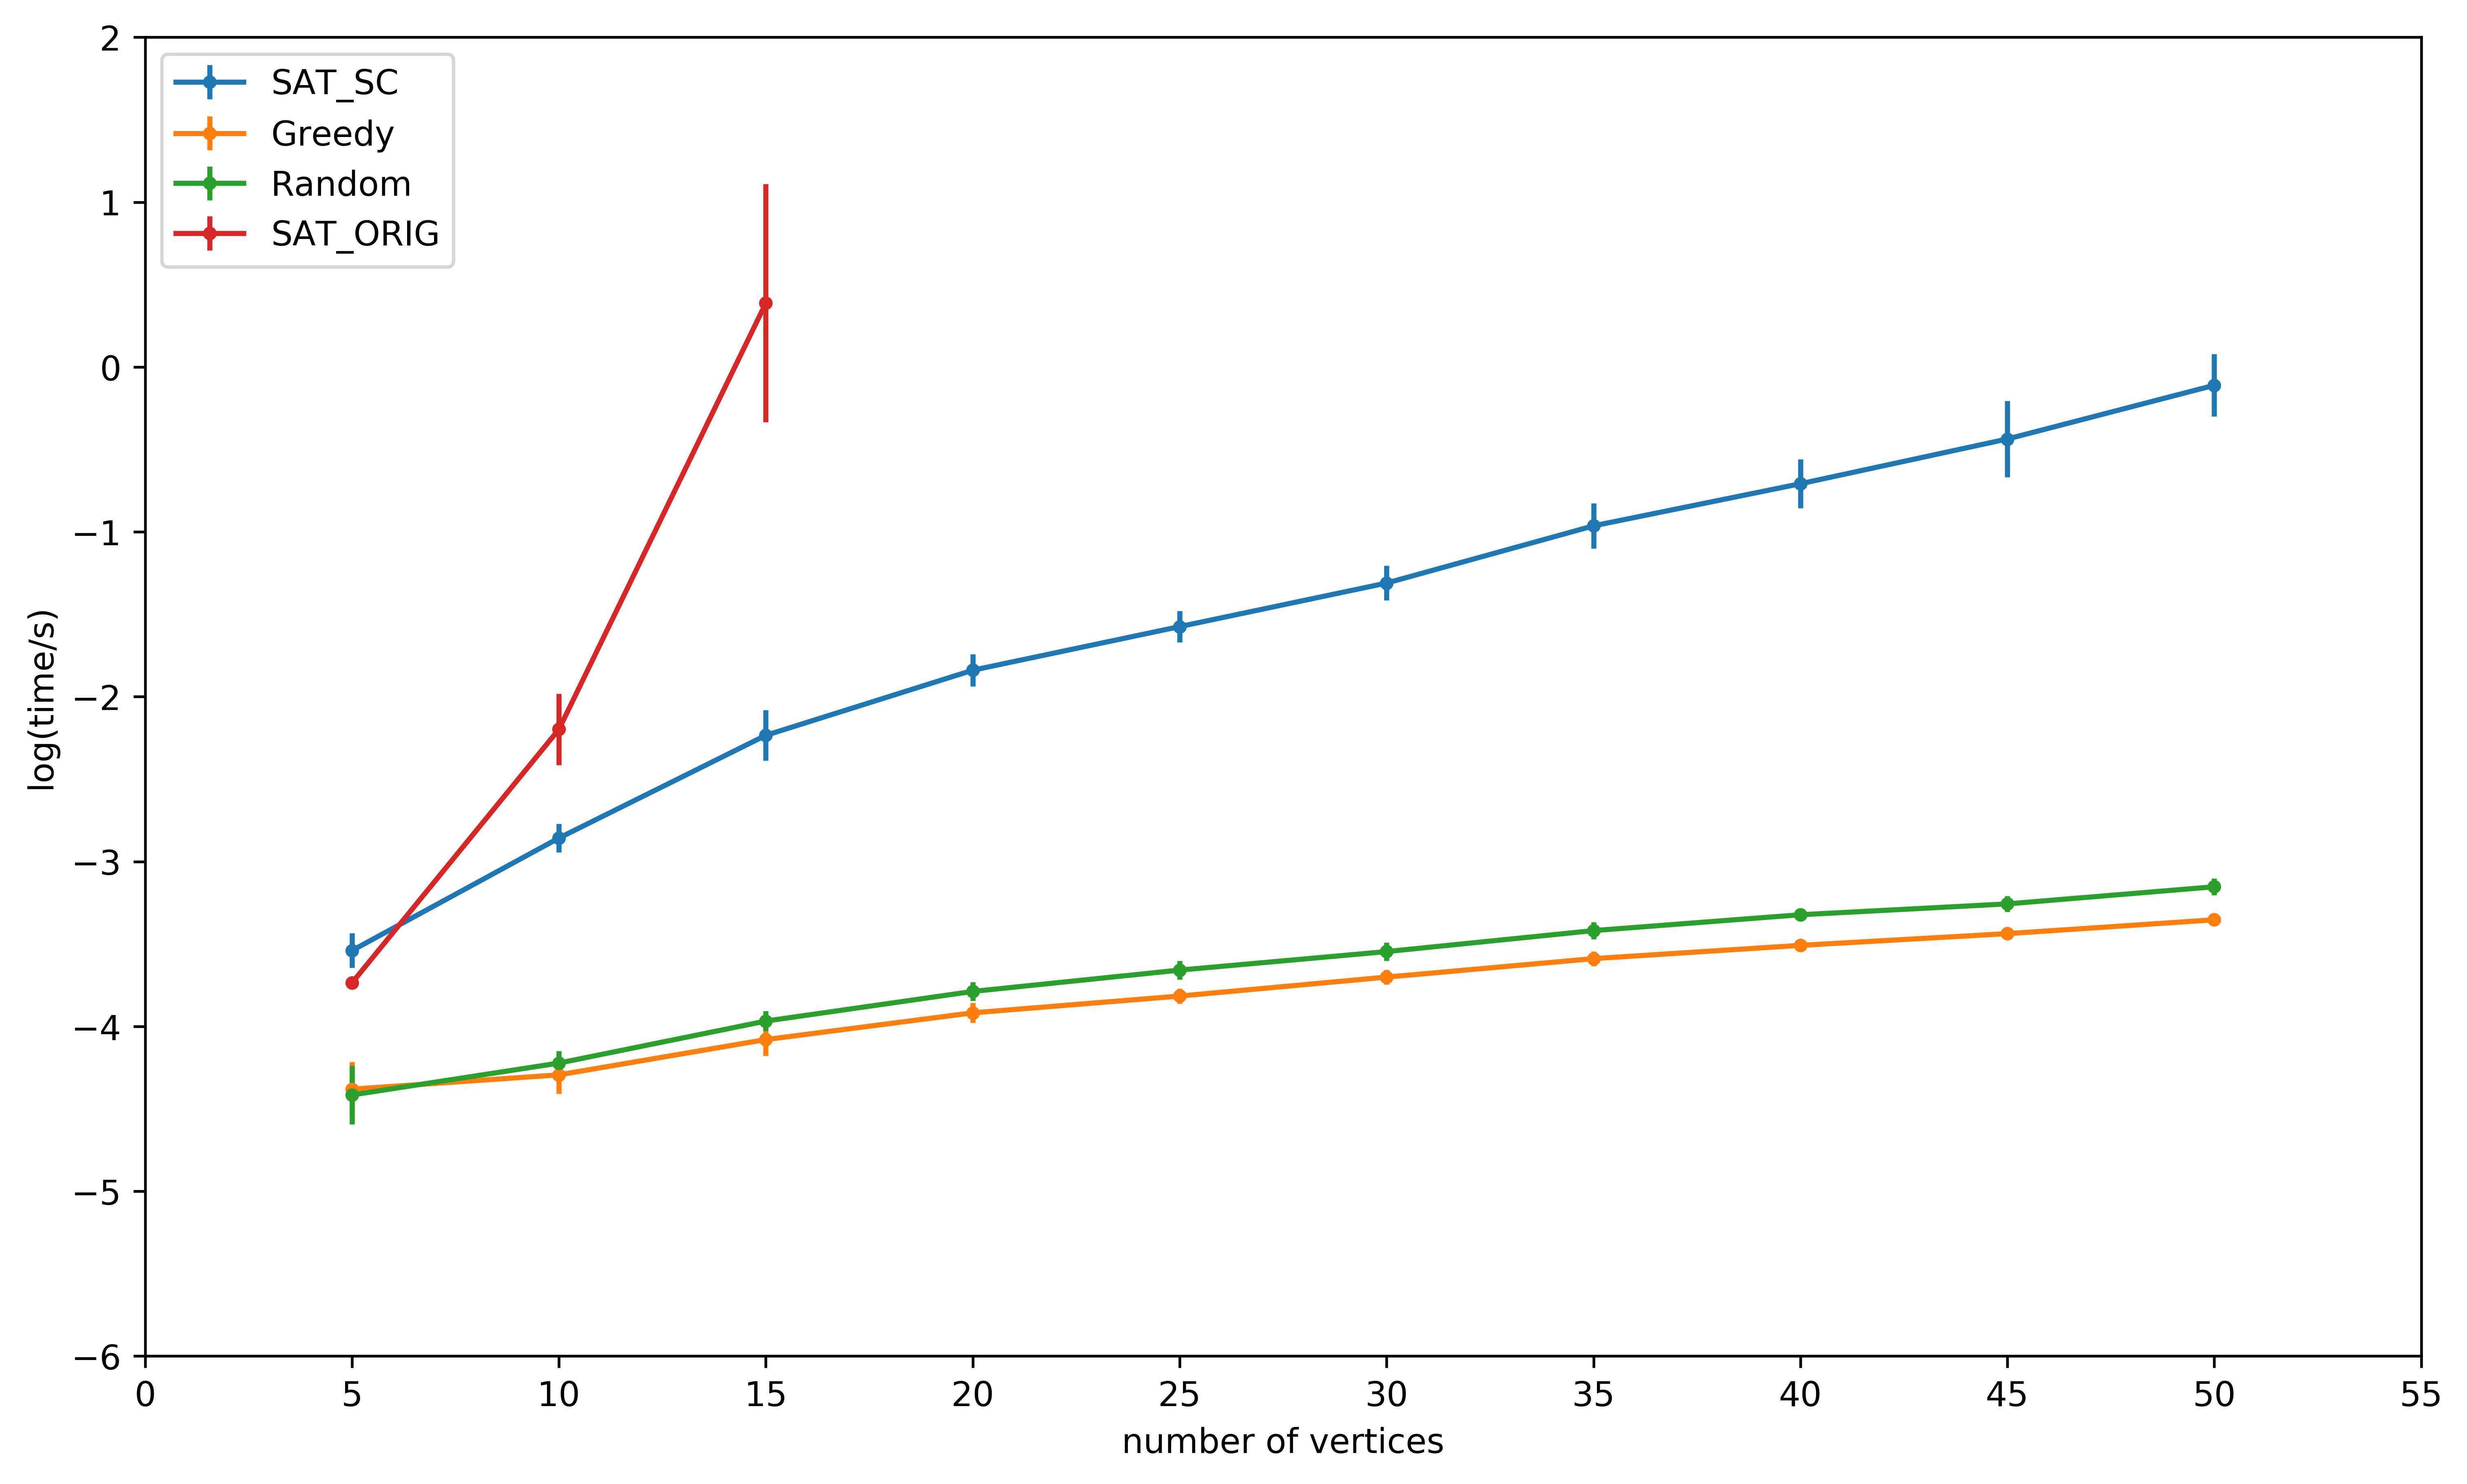
\includegraphics[width=13cm]{time_sc_slow.png}}
\caption{Log Run Time of the Four Algorithms}
\end{figure}
Figure 3 shows the log running time of the algorithms vs the graph size. In the plot, $\textsc{SatOrig}$ refers to the exact algorithm with encoding in ece650.a4. The $\textsc{SatSC}$ refers to the exact algorithm with sequential counter encoding. 

The slope of $\textsc{SatOrig}$ and $\textsc{SatSC}$ is relatively large, indicating $miniSAT$ uses algorithm with exponential running time. There is a huge performance gap between $\textsc{SatOrig}$ and $\textsc{SatSC}$ due to different encodings of the same problem. The former times out when $n \geq 20$ while the latter could handle an input of at least 50 vertices. Another difference between these two encodings is their standard deviation. $\textsc{SatOrig}$ has a much larger standard deviation, which means for different graphs with the same number of vertices, the running time varies a lot, which also indicates this kind of encoding will generate much more clauses as $k$ grows: for a fixed vertex number $n$, it will take less time if a graph is dense. But if the graph is sparse, the original encoding will make $miniSAT$ run for a much longer time. This is not a big problem for the sequential counter encoding.

The slope of the two approximate algorithms is relatively small, indicating polynomial time algorithms. And both of them are faster than the exact algorithm in tens of orders. 

\begin{figure}[H]
\centerline{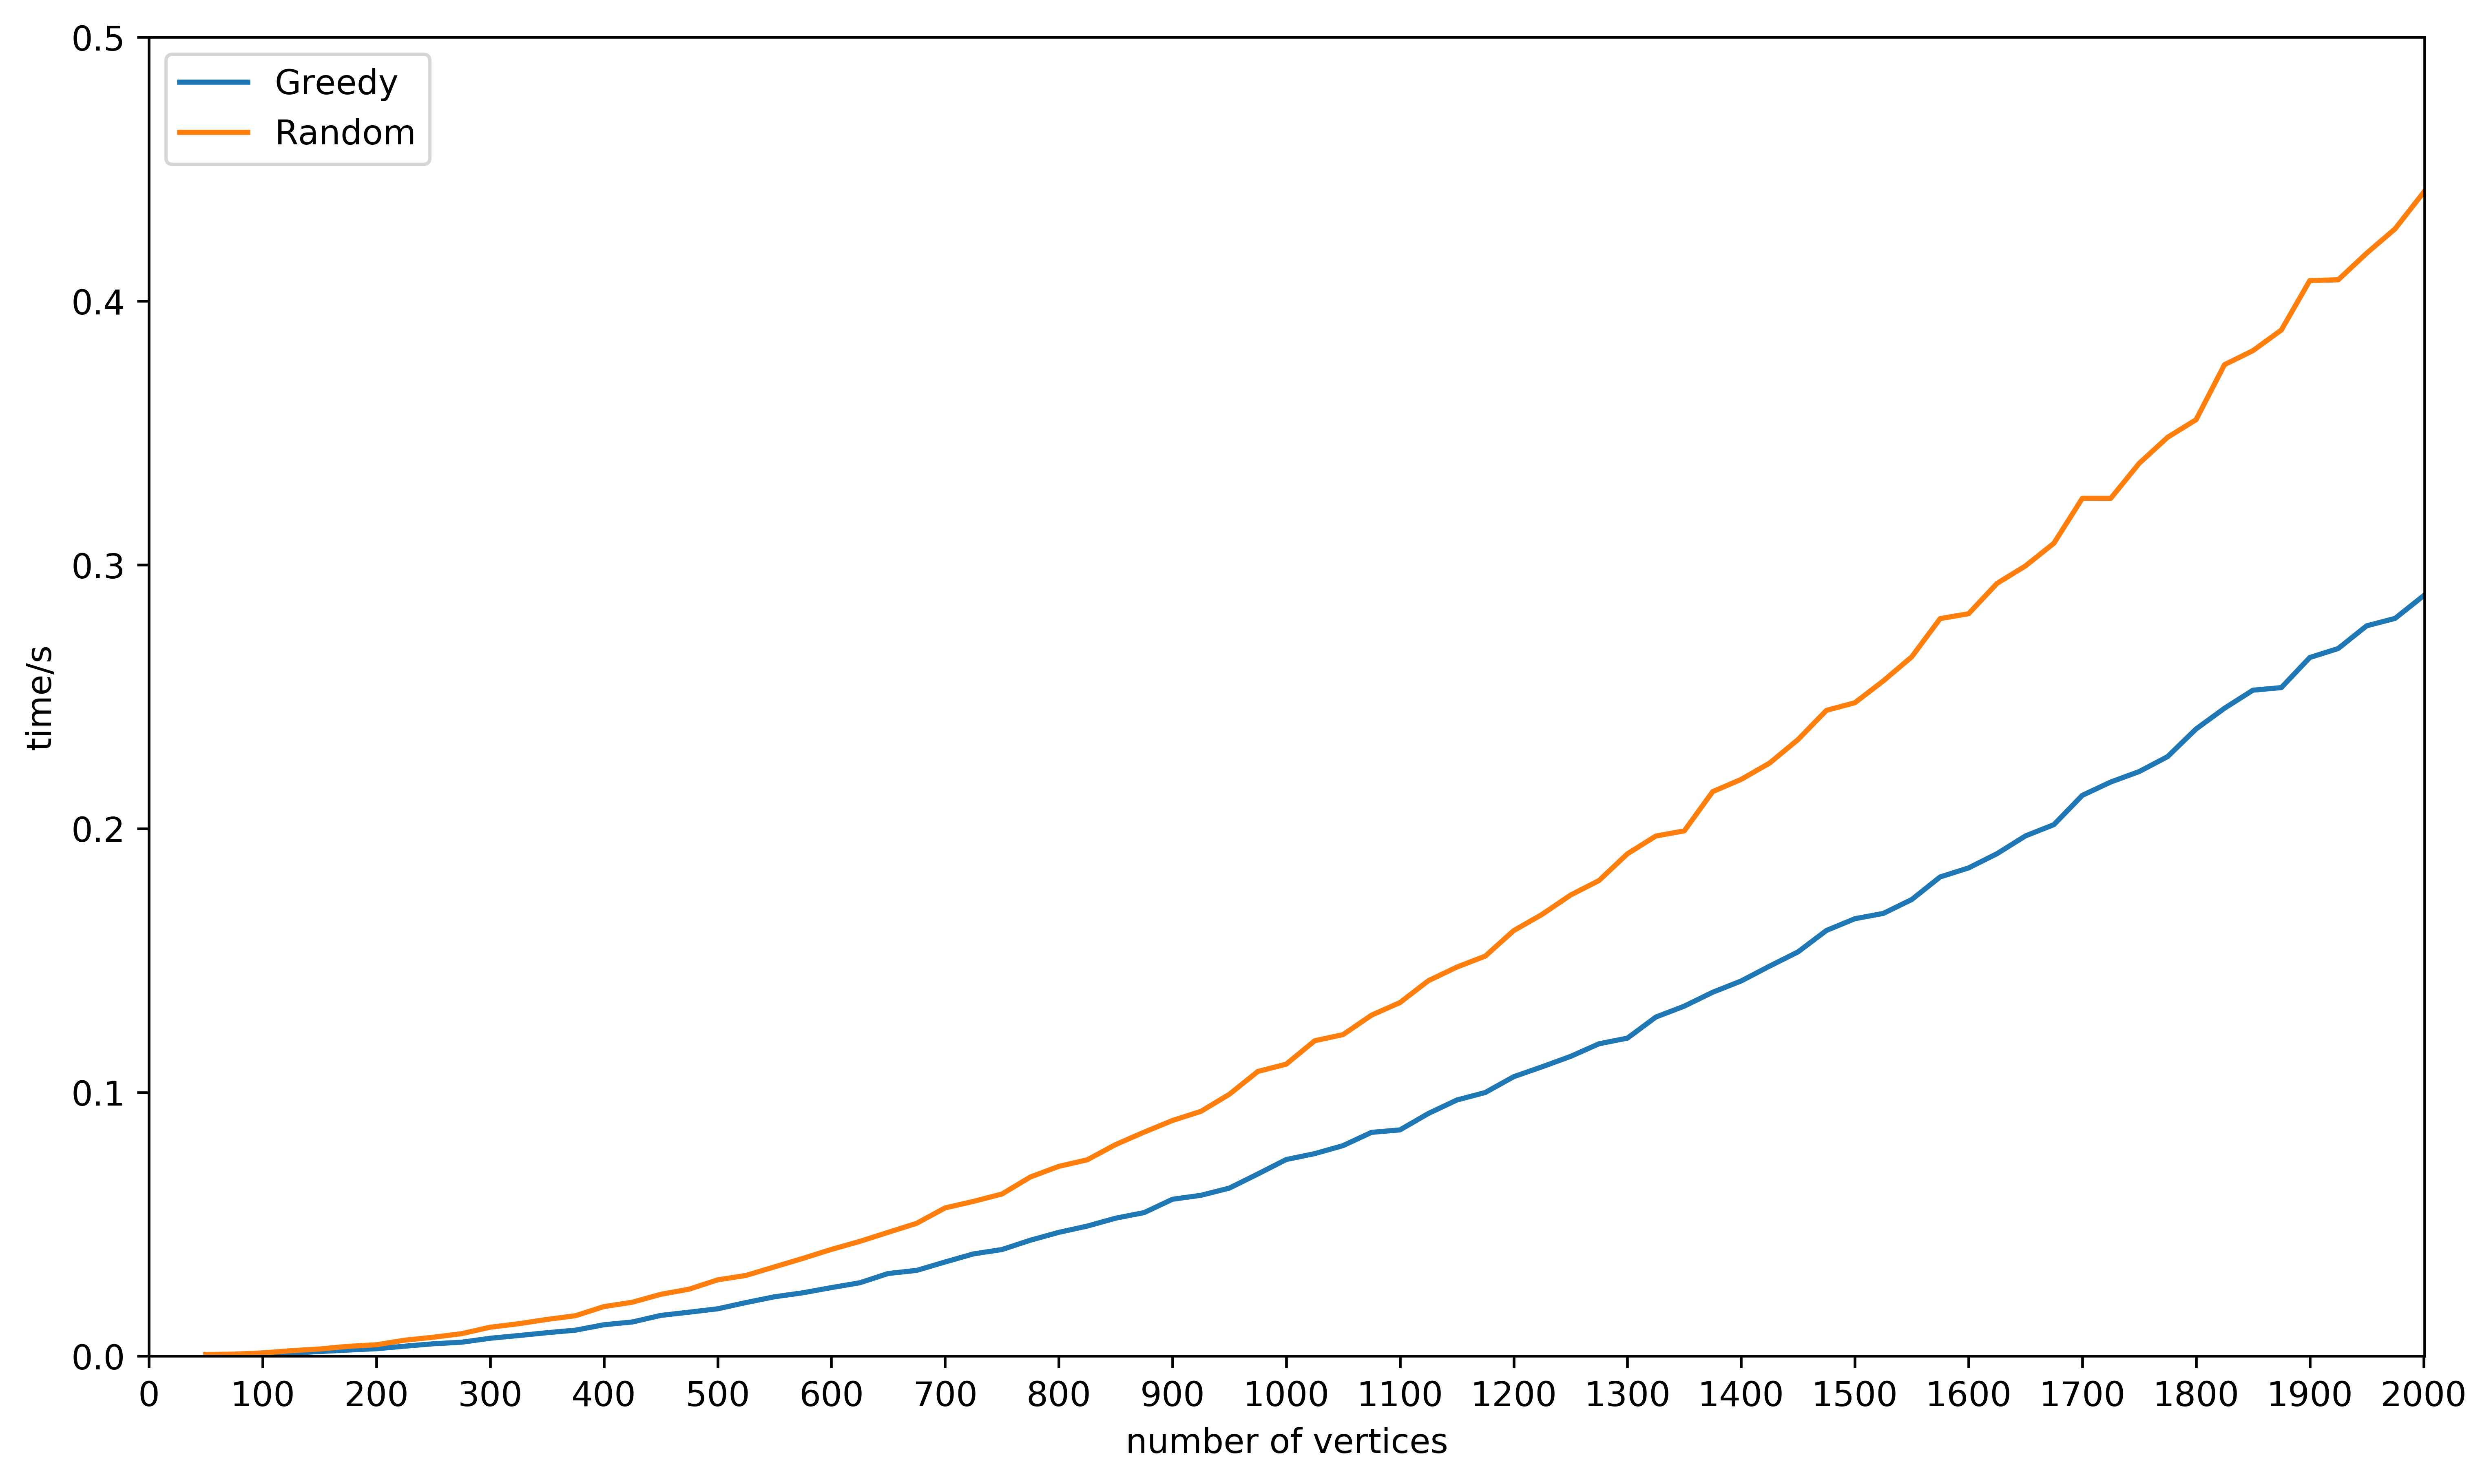
\includegraphics[width=13cm]{large_time.png}}
\caption{Run Time of the Two Approximate Algorithms}
\end{figure}

Figure 4 shows the run time of them when $n$ becomes larger. The greedy algorithm is still faster than the random, which may due to the adjacency list implementation of the graph. We cannot pick an edge directly, instead, we can only pick a vertex randomly and then pick another vertex in its adjacency list, which may slow down the algorithm.

\begin{figure}[H]
\centerline{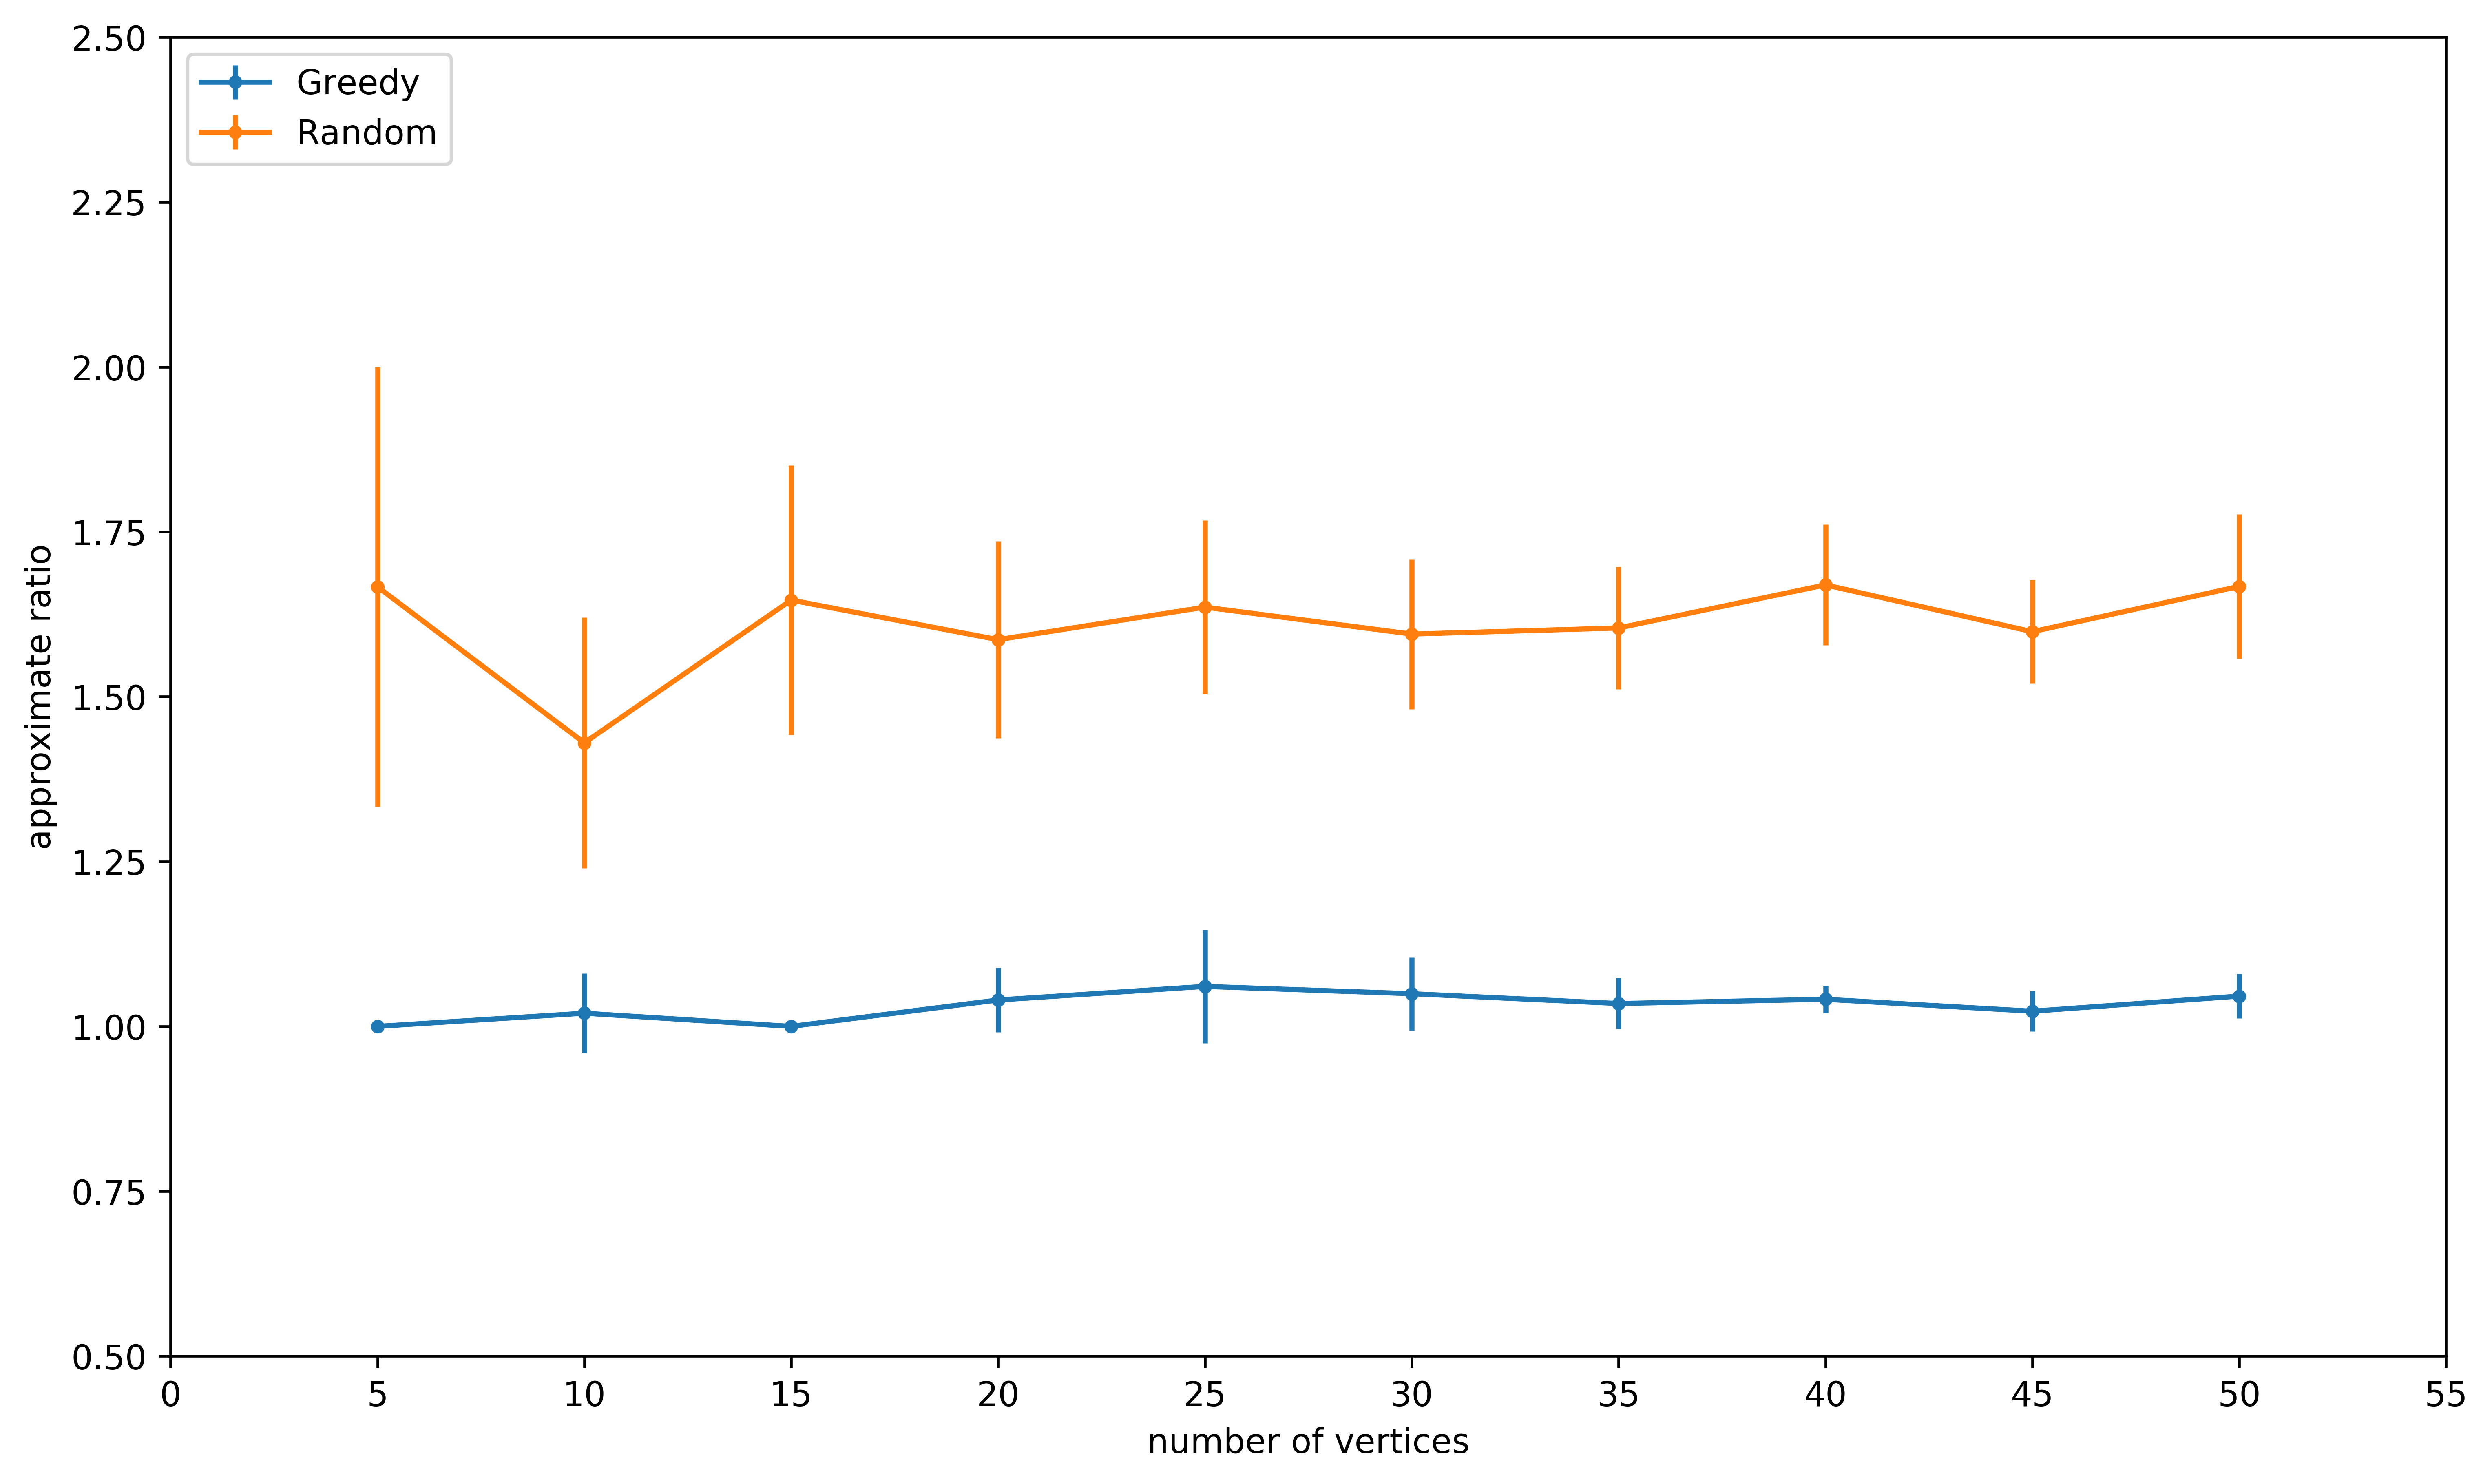
\includegraphics[width=13cm]{approx_sc.png}}
\caption{Approximate Ratio of Greedy and Random Algorithm}
\end{figure}
\begin{figure}[H]
\centerline{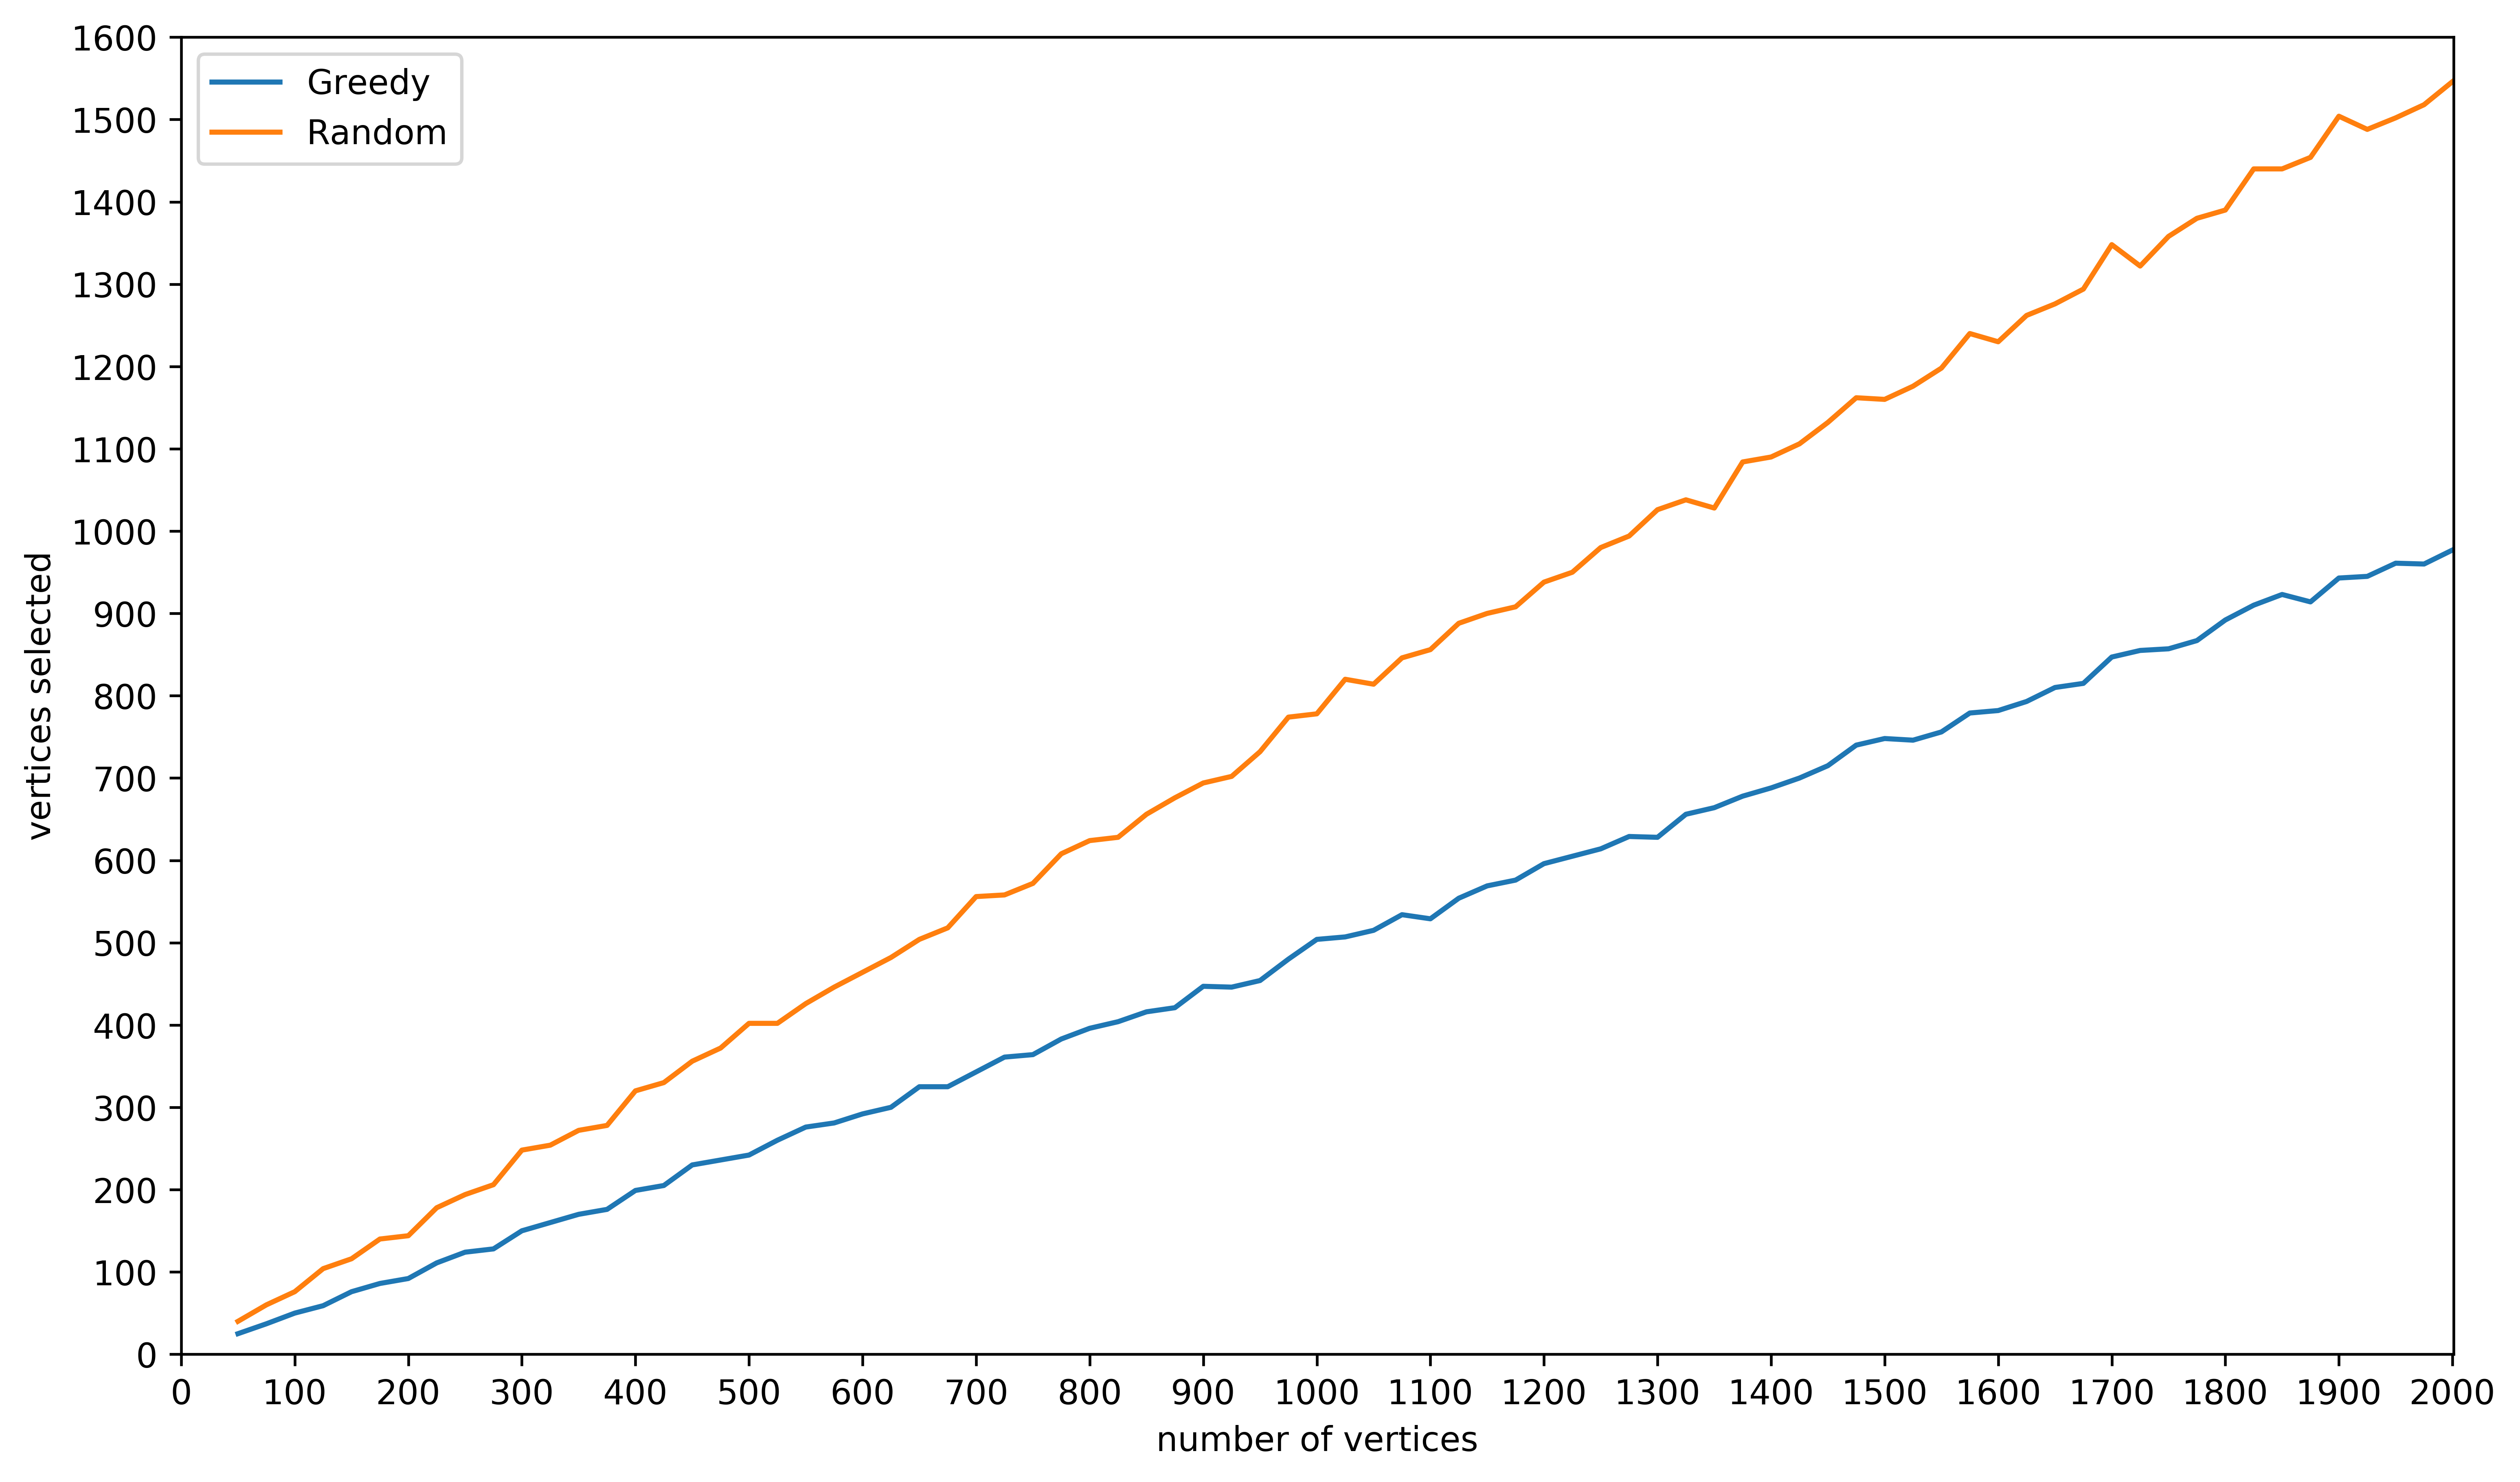
\includegraphics[width=13cm]{large_ratio.png}}
\caption{Approximate Ratio of Greedy and Random Algorithm ($n\leq2000$)}
\end{figure}

Although in theory, as shown in Chapter 4, the random algorithm has a better appromimate ratio (2) than the greedy algorithm ($\log(n)$), the greedy algorithm outperforms the random one in practice, with an approximate ratio slightly greater than 1, while the random algorithm is about 1.5. As currently the $n=50$ is not large enough, we cannot conclude which algorithm is indeed better than the other one. When $n$ becomes larger, although we cannot calculate the approximate ratio as the exact algorithm takes too long, we can still compare the number of vertices both algorithm selected, as shown in figure 6. We can say at least when the input graph is small($n<2000$), the greedy algorihtm is a better choice for an approximate solution.

\section{Conclusion}\label{section-conclusion}
In this paper, we explored two different encodings of reduction from Vertex Cover Problem to CNF-SAT problem. We reached a conclusion that the sequential counter encoding is better than the original encoding in terms of the clauses they produce, which will affect the performance of the CNF-SAT solver. We also compared them with two approximate algorithms, and we found for a small graph($n<2000$), the greedy algorithm is a better choice for approximation, with a lower approxiamte ratio than the random algorithm.

\bibliography{references}
\end{document}
